\documentclass{article} % For LaTeX2e
\usepackage{nips13submit_e,times}
\usepackage{hyperref}
\usepackage{url}
\usepackage{graphicx} 
\usepackage[caption=false,font=footnotesize]{subfig}
\usepackage{amsmath}
\usepackage{amssymb}
\renewcommand{\figurename}{\bf Figure}
%\documentstyle[nips13submit_09,times,art10]{article} % For LaTeX 2.09


\title{Biometric in Motion: Identification Using Acceleration Data}


\author{
Zexi Mao\\
\texttt{zexim@andrew.cmu.edu} \\
\And
Siqi Tan \\
\texttt{siqitan@andrew.cmu.edu} \\
\AND
Yuchen Wu\\
\texttt{yuchenw@cs.cmu.edu} \\
\And
Yimeng Zhang \\
\texttt{yimengzh@cmu.edu} \\
}

% The \author macro works with any number of authors. There are two commands
% used to separate the names and addresses of multiple authors: \And and \AND.
%
% Using \And between authors leaves it to \LaTeX{} to determine where to break
% the lines. Using \AND forces a linebreak at that point. So, if \LaTeX{}
% puts 3 of 4 authors names on the first line, and the last on the second
% line, try using \AND instead of \And before the third author name.

\newcommand{\fix}{\marginpar{FIX}}
\newcommand{\new}{\marginpar{NEW}}

\nipsfinalcopy % Uncomment for camera-ready version

\begin{document}


\maketitle

\begin{abstract}
The purpose of this project was to develop a method for classifying users of devices based on acceleration data and to discuss how to identify users without leaking their privacy. Raw acceleration data was segmented based on timestamp. Re-sampling was performed to unify the format of samples. After the preprocessing steps, six sets of features were extracted from raw and re-sampled data. For the classification task, three classifiers (k-NN, SVM and logistic regression) were applied. The best performing classifier got 0.907 area under the ROC (Receiver Operating Characteristic) curve. A quantitative analysis of user privacy issue was conducted based on types of features extracted and amount of data used.
%As cellphones and other smart devices are closer to our daily life than ever, we are curious to know how the data gathered by accelerometers on them impact our lives, particularly in terms of identifying users of devices via such data. In this project, we try to answer this question with machine learning techniques. We first studied how to implement such biometric techniques by retrieving useful identification information from raw accelerometer data. We then built classifiers with these information. At last we investigated in what way and how much of our privacy leaks through this technique via cellphones. We hope this work could show how such techniques impact our lives.
\end{abstract}

\section{Introduction}

\subsection{Motivation}

Ubiquitous computing had never been so close to us as our phones become smarter and more powerful today. Sensors equipped in our cellphones like GPS, gyroscope, accelerometer and even barometer collect data from the surrounding environment and ourselves. This information collected from our cellphones and other mobile devices can boost many more applications than just adjusting the brightness of the screen and rotating it automatically. Google uses the GPS data from our phones to provide real-time traffic conditions. Apps can track how well you sleep by just putting your phone beside you on bed. Indoor localization takes advantage of wireless fingerprint, sound from microphone, footsteps from accelerometer and even colors from the camera to tell you where you are when GPS signal is weak inside buildings. Fancier applications far beyond the original purposes of these sensors are on the way. How to retrieve more information from the raw sensor data is one of the hottest and promising topics today.

Accelerometer is one of the most interesting sensors in our cellphone, which records the acceleration data in 3D. Posture of the phone, gestures and footsteps of the user, and even the user's sleeping condition can be measured by the accelerometer.

In this project, we tried to explore a novel usage of the accelerometer: biometric identification. In other words, can we identify the user by only looking into how he (she) moves? We believe that everyone has his (her) own unique pattern of movement. If this assumption is true, we can identify the person when we match the current data from the accelerometer with the historical data we have learned. 

In this project, we chose the already available accelerometer dataset gathered by Kaggle. Due to the poor quality of the raw data set, we first performed preprocessing. The goal of preprocessing is to normalize data for easier feature extraction. Then we extracted discriminative features from the preprocessed dataset. The features we used included frequent domain patterns, relative and absolute time domain relations. We applied several classifiers to the feature vectors. So far, we have got a score of over 0.90 in terms of area under the ROC curve, which is satisfactory, although further improvement is still needed.

Furthermore, we studied how the features we used impacts the accuracy of identification. We also showed the relation between quantity of training data and accuracy. These results help us understand what leaks our private information and how to stop it.






\subsection{Related Work} 

A human being's walking gait can reflect the walker's physical characteristics and psychological state, and therefore the features of gait can be employed for individual recognition. The use of accelerometer data for biometric identification is relatively new but has been increasingly explored in recent years. Existing methods for gait recognition have shown good performance.
 
Gafurov et al. \cite{Gafurov:AIAT2007} attach multiple sensors to a subject at different body parts. Xu et al. \cite{Xu:ICB2012} developed an Android App to collect gait acceleration data. With a reasonably sized dataset, by matching gait patterns across different paces, they show preliminary results indicating that not only can smart phones be used to identify a person based on their normal gait but also that there is potential to match gait patterns across different speeds.

Tao et al.\cite{Tao:ToPAMI2007} focus on the representation and pre-processing of appearance-based models for human gait sequences. Two major novel representation models are presented, namely, Gabor gait and tensor gait. Experiments show that the new algorithms achieve better recognition rates than previous algorithms.

Pan et al. \cite{Pan:EL2009} proposed algorithm based on signature points, instead of the whole gait signal. They consider acceleration-based gait recognition insensitive to changes of lighting conditions and viewpoint. Their algorithm firstly extracts signature points from gait acceleration signals, and then identifies the gait pattern using a signature point-based voting scheme. The experimental results shows the accelerometer-based gait biometrics is promising. 

Kwapisz et al.\cite{Kwapisz:BTAS2009} collect some data and also perform identification experiments . Based on the 600 raw accelerometer readings, they generated 43 features, which are variations of 6 basic features including average acceleration value, standard deviation, time between peaks and so on. They applied two classification techniques decision trees neural networks to classify and the identification performance turned out to be fairly good.


\section{Information on the Kaggle Competition}
\subsection{Raw data}
The dataset provided by the Kaggle competition \href{http://www.kaggle.com/c/accelerometer-biometric-competition}{``Accelerometer Biometric Competition''}. The dataset consisted of 3 parts: a training set, a testing set and a question set. Each single sample point in training and testing sets contained a time stamp in milliseconds, acceleration measurements in 3 dimensions, and an associated DeviceId (for the training set) or a SequenceId (for the testing set). 

In the training set, there were 30 million samples, which were collected from 387 different devices as labeled. These samples were demarcated into 387 segments, each containing samples for a single device. In the testing data set, there were also about 30 million samples without label. These samples were demarcated into 90,024 sequences of 300 points, each with a SequenceId. In the question set, for each SequenceId, there was a proposed DeviceId.

\subsection{Evaluation}
The task on Kaggle was to tell whether each sequence's proposed DeviceId was the sequence's real DeviceId. For each sequence, we were required to give a belief, in real number, about the credibility of the proposed DeviceId. This competition was designed to investigate the feasibility of using accelerometer data as a biometric for identifying users of mobile devices. For more detail, please refer to the competition website as listed above.

We should emphasize our goal of this project is not simply performing well in the Kaggle competition, but aims at how such technique impacts our daily life. However, for fairly evaluating our approach, we use the Kaggle online judging system along with hundreds of other teams. This system automatically outputs the area under the ROC curve as the score for a submitted answer generated by our classifiers. 


\section{Methods}
In this section, we describe the methods we used for preprocessing, feature extraction, and classification.


\subsection{Preprocessing}
Two problems with the raw dataset need to be tackled before further processing: 1) the accelerometer data for each device was not properly segmented; 2) the accelerometer readings were not uniformly sampled according to the timestamp. Regarding these problems, segmentation and re-sampling were performed respectively.

\begin{figure}
    \hspace{-0.5cm}
    \begin{minipage}[t]{0.02\textwidth}~
    \end{minipage}
    \begin{minipage}[t]{0.47\textwidth}
    \centering
    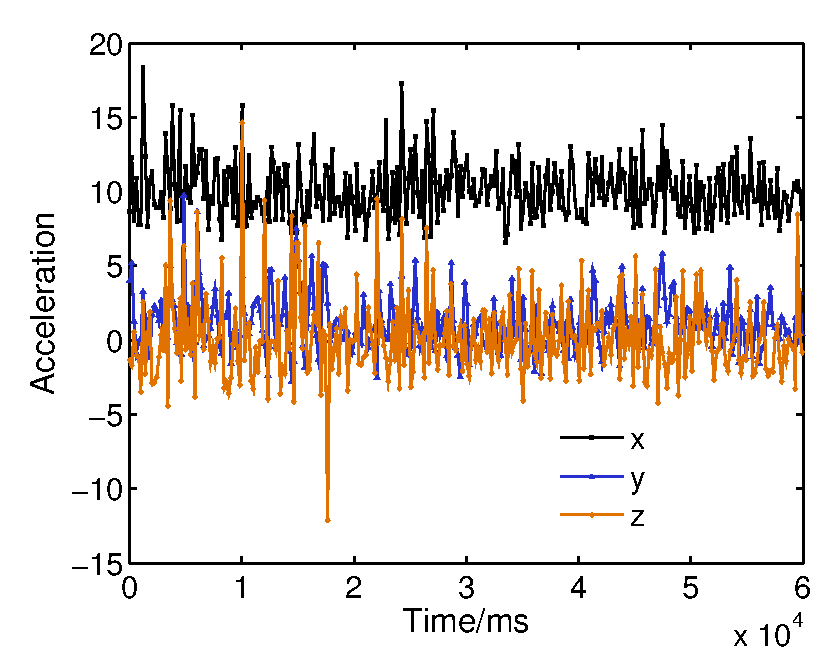
\includegraphics[height=40mm]{fig/good_raw.eps}
    \caption{Example of a good sequence from raw data: samples points are close in time. These points are regarded as representing a single activity.}
    \label{fig:good_raw}
    \end{minipage}
    \begin{minipage}[t]{0.02\textwidth}~
    \end{minipage}
    \begin{minipage}[t]{0.47\textwidth}
    \centering
    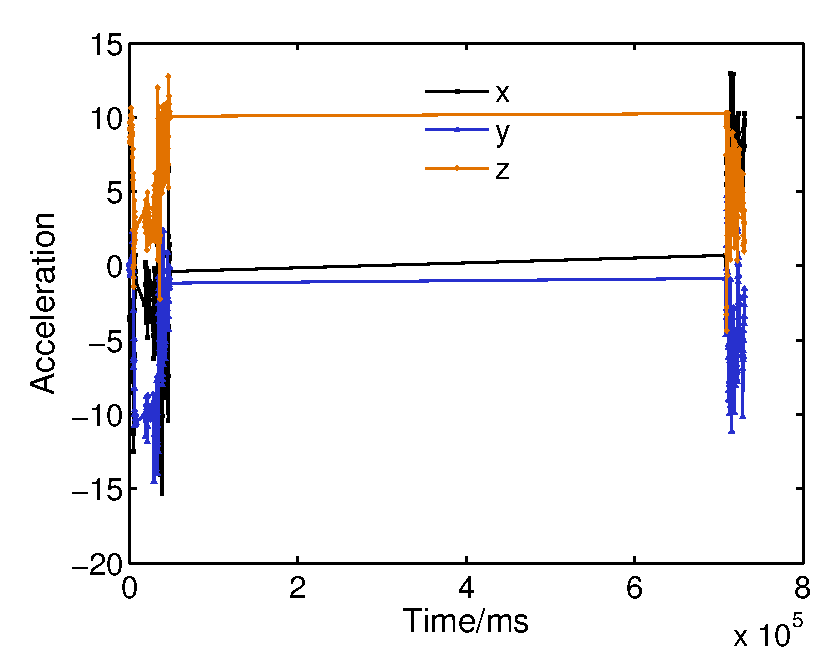
\includegraphics[height=40mm]{fig/bad_raw.eps}\\
    \caption{Example of a bad sequence from raw data. This piece essentially contains information about two separate activities that are far apart in time. The line segments in the middle of the figure was due to the large time intervals between adjacent sample points.}
    \label{fig:bad_raw}
    \end{minipage}
    \begin{minipage}[t]{0.02\textwidth}~
    \end{minipage}%   
 \end{figure}


\subsubsection{Segmentation} % (fold)
For each sequence of acceleration samples in the raw data, the time intervals between two adjacent sample points are less than 500ms for most of the time. However, some intervals can be as large as 100,000ms. This problem is illustrated in Figures \ref{fig:good_raw} and \ref{fig:bad_raw}. They both contain two test sequences of 300 points. In the first sequence (Figure~\ref{fig:good_raw}), all sample points are close in time, and we can treat these points as representing a single activity. In the second sequence (Figure~\ref{fig:bad_raw}), there are two points with a large time difference (so all the other points are pushed to two sides of the figure). Thus, we can consider this sequence containing information about two separate activities. 

It shoule be clear that we cannot consider the second sequence as representing a single activity, since so much information is missing between the two far apart sample points. Such huge time interval is not uncommon in the dataset. %This could be attributed to two reasons: 1) in preparing this dataset, sequences of samples during periods of rest exceeding 10 seconds were removed by Kaggle; 2) the device could be off or the app could be closed during the whole data collection process. 

To tackle this problem, segmentation was performed on the raw data to split each sequence into subsequences. The segmentation has two phases. In the first phase, we split the sequences that have time intervals larger than $T_\mathrm{split}$. After that, shorter subsequences with sample points close in time. In the second phase, we continually split the longest subsequence among all the subsequences until 1) we got $k_\mathrm{\#seq}$ subsequences, or 2) the longest subsequence was shorter than $2 l_\mathrm{maxL}$. Also, sequences shorter than $T_\mathrm{short}$ were thrown.

We did the second-phase segmentation because after the first-phase segmentation, some resultant sequences were too short (less than 1000 ms) so that not much reliable features could be extracted, and some were too long (longer than 100 seconds) so that it might contain information about multiple activities of the user. 

In this manner, on the one hand, we make more sequences from one device, hopefully keeping more information about the device's diverse patterns. On the other hand, we keep the sequences long enough, so that they contain reliable information about patterns of the device.

\subsubsection{Re-sampling} 
After segmentation, for each device, we got several subsequences. However, these sequences were not uniformly sampled, due to various reasons. To make feature extraction simpler, we interpolated each segment using cubic spline and uniformly re-sampled each sequence with  $\tau_\mathrm{resample}$ being the re-sampling time interval.

\subsection{Feature extraction}
\label{feautures}

After preprocessing, for each raw sequence (from training set or testing set), we got several shorter re-sampled subsequences. In this section, we describe how to extract features from each subsequence.
	
%In the end, for each subsequence, we got a feature vector in $\mathbb{R}^{1290}$. This vector can be decomposed into 3 parts: frequency domain features, time domain features, and accelerometer reading features.
Six categories of features were investigated. They represent different aspects of patterns from the data.

\subsubsection{Frequency domain features}
As different people has their own pace for actions, we believe the patterns of human mobility can be easily exploited in frequency domain. To this end, for each subsequence, we first extracted sliding windows of size $w_\mathrm{fft}$ and 50\% overlap (features extraction on windows with 50\% overlap has demonstrated success in previous work \cite{Bao:PC2004}). Then we did FFT on all windows. Finally, we calculated the magnitude of all first $(w_\mathrm{fft}/2 + 1)$ coefficients and used the average values over all windows as the frequency domain features for the subsequence. Because readings were from 3 directions, we have $(w_\mathrm{fft}/2 + 1)\times 3$ values for frequency domain features per subsequence.

\subsubsection{Differences of acceleration}
More patterns and properties were discovered when we look beyond frequency domain. One obvious feature is the absolute difference between two adjacent readings of acceleration \cite{Kwapisz:BTAS2009}. This feature measures how rapidly a person usually handles the phone or moves. It may also indicate the environment this person lives. The distribution of such differences was taken as the features in this category. Specifically, we computed three histograms (30 bins each histogram, edges of leftmost and rightmost bins determined by the 5\% and 95\% quantiles of absolute differences for each axis) of absolute differences between every adjacent pair of readings on three axes for each sequence as its features. 

\subsubsection{Resultant acceleration}
The value of each reading alone can also imply useful information. The resultant acceleration \cite{Kwapisz:BTAS2009}, which is defined as $\sqrt{x^2+y^2+z^2}$ ($x,y,z$ are readings at a particular time), directly evaluates the absolute value of the acceleration of the device. This value reveals how hard a person usually moves as the force is proportional to the acceleration it measures. The distribution of resultant acceleration is the third feature we used. Same as mentioned above, the histogram (prepared in the same way as the previous feature) of this value was produced for each sequence as one category of its features.

\subsubsection{Histogram of acceleration readings}
Inspired by the above features, distribution of acceleration readings each of three dimensions can also be informative. For example, a phone may lie on a desk if the reading of its reading for z axis (the axis perpendicular to the screen) is more likely to be 9.8 $\mathrm{m}\cdot \mathrm{s}^{-2}$ (gravity), while another phone's reading for y axis is larger when it is always kept in one's pocket. Three histograms (prepared in the same way as the previous two features) were generated for every sequence.

The above four sets of features were what we mainly focused on. There were also many tricky features which could help us a lot to have a better score in the competition. However, these features could be useless in real world applications. 

\subsubsection{Raw sampling rate}
As the mobile devices people use are increasingly diverse, the characteristics of different devices offer us a set of very distinguishing features for recognizing users. One of these characteristics was the sampling intervals of the devices.

As we observed from the raw data set, sampling intervals of devices has a range of approximately 5-250 ms, and for different devices, the distributions of the sampling intervals were quite different. Thus, for each subsequence, we used the histogram (0-600 ms divided into bins of 20 ms, in total 30 values) of the sampling intervals of the original sequence it came from as the time domain features. 

\subsubsection{Sampling granularity}
Apart from the sampling intervals of devices, we found another set of features with potential ability of distinguishing devices, which was the accelerometer readings.

By observing the data, we found that each kind of device could only provide certain discrete values of accelerometer readings, and this might be due to the limited precision of accelerometers. Thus, the set of accelerometer readings a device can provide is also treated as a set of features. For each subsequence, we calculated the overlap between the the set of readings from the original sequence it came from and the set of readings from the $i$th device, $i=1,\ldots,387$. Since we had readings from 3 directions, $3\times 387 = 1161$ values constituted the accelerometer reading features for each subsequence.

The two tricky features introduced above help teams to gain satisfactory scores in the Kaggle competition. However, they focus more on classifying devices rather than users. They could easily fail in real world when a large amount of people use the same type of devices such as iPhones. These features may also fail when a person uses several devices at the same time or switches to a new device.

\subsection{Classification}

Once the key features are extracted, we move on to leverage various kinds of classifiers and optimize their parameters for more accurate results.

After preprocessing and feature extraction, for each original sequence, we now had several feature vectors associated with it. These vectors were used for classification. For each vector, we let the classifer output the probability (belief) that it comes from device $i$ ($i=1,\ldots,387$). Then, the average of beliefs of all feature vectors associated with a test sequence on the proposed DeviceId was used for submission.

We started from some naive classifiers. The performance of K-nearest-neighbor depends on the number of K and the definition of distance function. This classifier gave us a baseline result. Then we moved on to popular classifiers such as support vector machines and logistic regression. We will also investigated the impact of the parameters of these classifiers in the following sections about implementation.


\section{Implementation and Evaluation}
In this section we show how our approach performed. We will justify the selection of parameters for preprocessing. We will also show the impact of quantity of training data and different features on results. We hope this could tell us how much training data is required to achieve an acceptable performance, and more importantly, how to prevent leakage of our identity by controlling what kind of accelerometer data to use.

\subsection{Evaluation methods and metrics}
We used the online judging system of Kaggle for fairness. It could also demonstrate how our approach performed against other teams all over the world. 

The system took results generated from our classifier as input. Then, the system produced value of area under the ROC curve (AUC) as the score. The baseline of AUC is 0.5 which stands for purely random guesses. A higher AUC value means a better classifier. A result with AUC of 1 stands for perfect guess. 

\subsection{Parameter selection}
In this subsection we discuss how to determine the parameters and thresholds we defined in the previous sections.


\subsubsection{Default values}
$T_\mathrm{split}$ was set to be 10 seconds to be consistent with the preprocessing setting done by Kaggle.  $T_\mathrm{short}$ and $l_\mathrm{maxL}$ were both set to be 4.8 seconds for the training set and 3.2 seconds for the testing set empirically. $\tau_\mathrm{resample}$ was set to be 200 milliseconds based on statistics of the distribution of the time intervals of the raw data, but any value near 200 ms should be a reasonable choice. The window size of FFT, $w_\mathrm{fft}$, was 64, which meant a window of duration 12.8 seconds. For training, $k_\mathrm{\#seq}=50$; for testing, $k_\mathrm{\#seq}=5$.

\subsubsection{Frequency domain granularity}
One of the important parameters is the number of samples for FFT. The resampling was taken at 200ms. So, FFT features describes the data’s frequency components from 0Hz to 1/0.2/2 = 2.5Hz. With original 64 point FFT, the frequency components are spaced at 2.5/32 Hz. 

However, such fine granularity in frequency domain (2.5/32 Hz between components) may not necessarily lead to better results. Some of these components can be highly correlated and so be redundant and even lead to worse performance. We wanted to investigate how the granularity of these features affect the performance. To do this, we first did 96 point FFT (48+1 featuress per axis) and 64 point FFT (32+1 features per axis) on each sequence. Then we downsampled these features by only keeping every 2-, 4-, 8-, and 16-th components, so that we had 10 different sets of FFT features for each sequence, covering the frequency from 0Hz to 2.5Hz, but at different granularities.


\begin{figure}
    \hspace{-0.5cm}
    \begin{minipage}[t]{0.02\textwidth}~
    \end{minipage}
    \begin{minipage}[t]{0.47\textwidth}
    \centering
    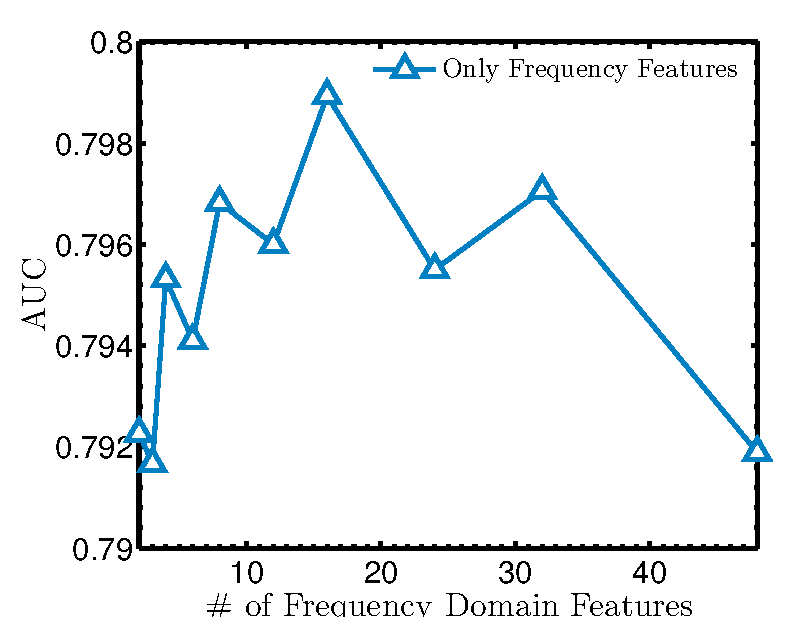
\includegraphics[height=40mm]{fig/fftauc.eps}
    \caption{AUC vs granularity of features in frequencey domain. Only frequency domain features are used with logistic regression.}
    \label{fig:FFTAUC}
    \end{minipage}
    \begin{minipage}[t]{0.02\textwidth}~
    \end{minipage}
    \begin{minipage}[t]{0.47\textwidth}
    \centering
    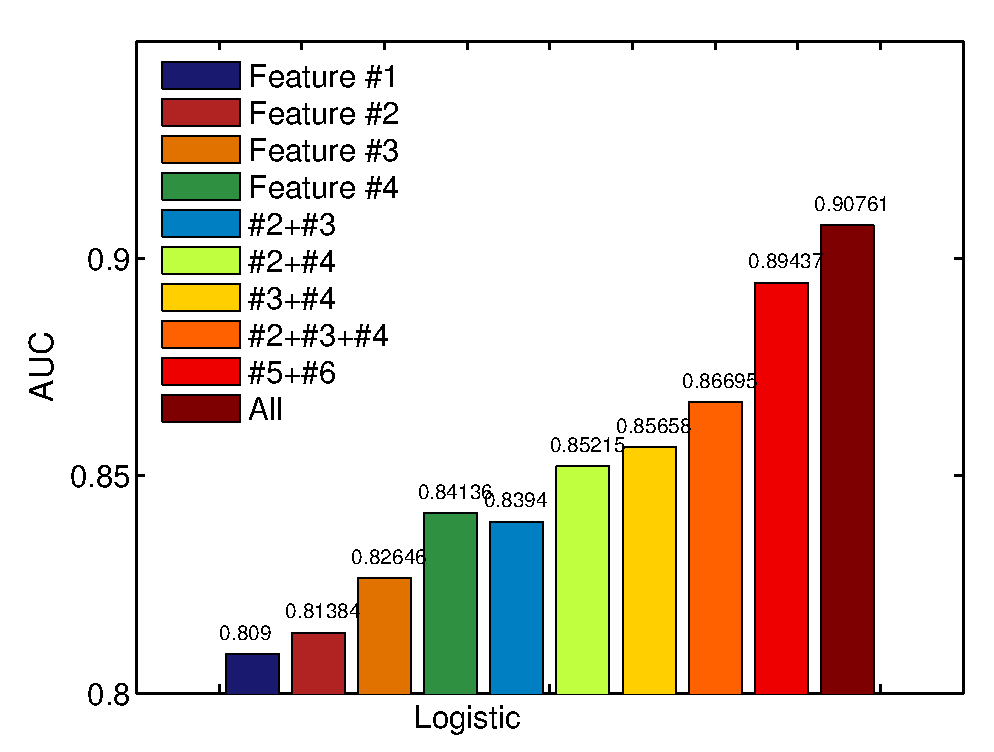
\includegraphics[height=40mm]{fig/feature.eps}\\
    \caption{AUCs vs combinations of features using logistic regression.}
    \label{fig:feature}
    \end{minipage}
    \begin{minipage}[t]{0.02\textwidth}~
    \end{minipage}%   
 \end{figure}

Figure \ref{fig:FFTAUC} shows the results for different frequency granularities. We only applied frequency domain features on logistic regression. The result indicates that feature vectors of length 17 to 33 perform better than smaller or greater ones on average. We can also find that neither smaller nor larger number of features performed significantly worse than the optimal ones. This fact means fine-grained feature extraction cannot exploit much more independent features than the coarse-grained ones. The reasons could be: 1) patterns of human movement do not have strong regularity on the frequencies (0 Hz to 2.5 Hz) we investigated. 2) accelerometer is not sensitive enough to gather that many useful features. 3) the features there are useful in theory, but noise due to accelerometer and other factors is also strong in that frequency range. If we have devices better than cellphone in terms of sensitivity and noise reduction, we may better explain this phenomenon.

Since there was no substantial difference for choices of granularity, in the following experiments, we just used 3 features (the shortest among all feature vectors we tested) for each axis as FFT features (also known as ``Feature \#1'').

\subsection{Tuning classifier}
Our preliminary results showed that L2-norm K-nearest-neighbor algorithm ($k=40$) leads to really poor results which achieved less than 0.6 in AUC. Although $k$ and the metric could be changed, we simply abandoned KNN for its poor performance and its time-consuming computation.

We use logistic classifier as one of our main options. The only parameter can be tuned in this classifier is $C$ (in LIBLINEAR) as the regularization parameter of logistic regression. It turns out that our features and data were not sensitive to the value of $C$ (no matter what combination of features used, AUC only fluctuated by about 0.0002). Therefore, we just used $C=1$.

We also tried support vector machine classifier. As it was very time-consuming, we only tested $C=1, \gamma=1$ (LIBSVM) for a SVM with a Gaussian kernel.

\subsection{Results}

Here we present the performance of our classifers. For convenience, we denoted the 6 kinds of features used as Feature \#1 to Feature \#6, corresponding the order they appear in the section of feature extraction. First, we show the performance of classifers using all 6 features. Second, results for different combinations of features are given. Last, results under different amounts of training data are shown.

\subsubsection{All features} % (fold)
\label{ssub:all_features}
Here, all resuls on reported using all 6 kinds of features, in Table \ref{tbl:test_result}.
% subsubsection all_features (end)

\begin{table}[!ht]
\caption{AUCs for different classifers, using all kinds of features}
\label{tbl:test_result}
	\begin{center}
		\begin{tabular}{ c | c  c  c  }
			\hline
			 Methods & L2-norm KNN & SVM & LR \\
			 \hline
			 AUC & 0.58302 & 0.80701 & \textbf{0.90761} \\
			 \hline
		\end{tabular}
	\end{center}
\end{table}


\subsubsection{Combinations of features} % (fold)
\label{ssub:combinations_of_features}
Results using different combinations of features are reported in Figure \ref{fig:feature}. Only logistic regression was used for classification.

% subsubsection combinations_of_features (end)


\subsubsection{The impact of amount of training data on performance} % (fold)
\label{ssub:the_impact_of_amount_of_training_data_on_performance}
Results using different amounts of training data are shown in Figure \ref{fig:percentage}. We reduce the size of training data by randomly selecting a portion of all training feature vectors, each vector corresponding to a split and re-sampled subsequence. Note that because Features \#5 and \#6 were not generated based on the subsequence, only Features \#1 to \#4 were used in this test. Again, only logistic regression was used.

\begin{figure}
    \centering
    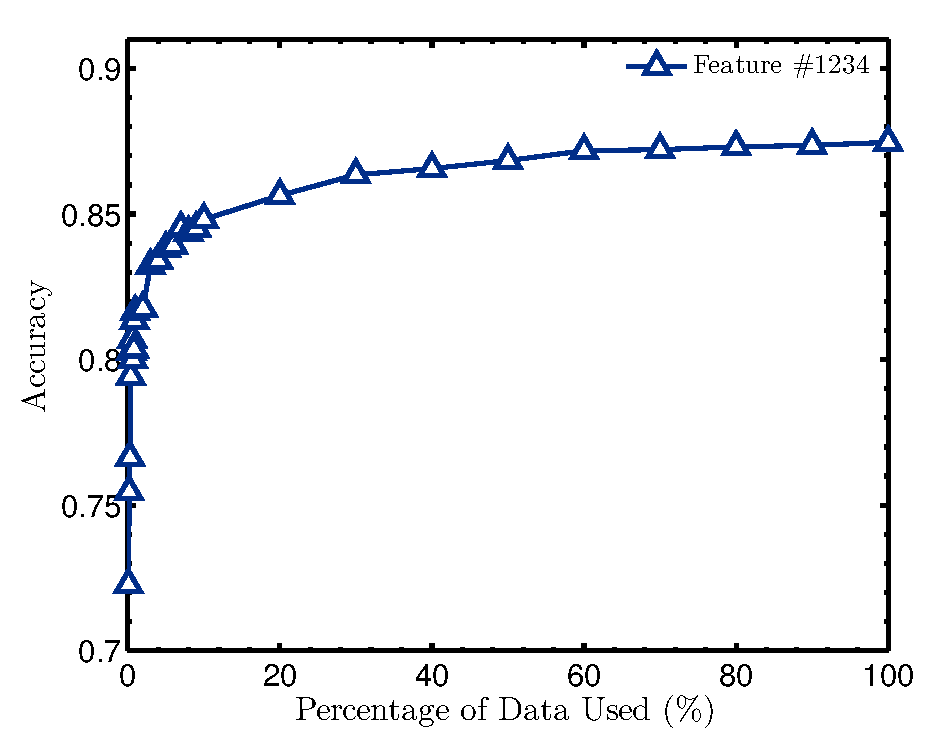
\includegraphics[height=40mm]{fig/percentage.eps}\\
    \caption{AUCs vs percentage of training data using logistic regression.}
    \label{fig:percentage}
 \end{figure}

% subsubsection the_impact_of_amount_of_training_data_on_performance (end)
\subsection{Miscellaneous results using SVM}  % (fold)
\label{sub:miscellaneous}
Because using SVM was very time-consuming, we only tested under several conditions, and the results are shown in \ref{tbl:test_result_SVM}.

\begin{table}[!ht]
\caption{AUCs for different conditions, using SVM}
\label{tbl:test_result_SVM}
    \begin{center}
        \begin{tabular}{ c | c  c  c  }
            \hline
             Features & All & only \#1 & \#1 + \#2 + \#3 +\#4 (10\% training data) \\
             \hline
             AUC & 0.80701 & 0.81406 & \textbf{0.85112} \\
             \hline
        \end{tabular}
    \end{center}
\end{table}

% subsection miscellaneous (end)

\subsubsection{Analysis} % (fold)
\label{ssub:analysis}

% subsubsection analysis (end)

The best results from our approach ranks top 8\% out of 634 teams on Kaggle. Although, the top teams reach over 0.99 of AUC for this competition, the tricky features mentioned in previous section boost the accuracy a lot. According to the online discussion, simply using tricky features to distinguish and identify sensors could achieve the ideal results. 


Although the competition became a game of cheating as it suffers from ``leaks'', as quoted from one of the best teams, we, who did not take effort to leverage leaks, show that reasonable features, which are obtainable in real world, also leads to promising results.


\section{Privacy Control}
In this section we look beyond the competition for a more meaningful and emergent topic, privacy. Results of our approach and others show that using acceleration information, the identity of a person could be easily leaked to others via the mobile devices surrounding us. Before anyone come up with evil ideas based on it, we are urgent to know how much data we can give out before our identities are compromised and in what form the data we provide is safer than other form.

Besides identity, exploiting the raw traces of acceleration make a person even more vulnerable as it could be used for localization with our without the help of GPS. We first investigate how the features impact the accuracy of identification. We assume that distributions like histograms is safer than the frequency domain features. The reason is the data after FFT is still invertible while it is much harder to recovery the time domain trace from histograms. 

The results are shown in figure\ref{fig:feature} and figure\ref{fig:feature_svm}. We use various of combinations of features for the evaluation. The number of features are consistent with the sequence in section\ref{feautures}. Feature \#1 is the frequency domain feature.  Feature \#4 has the best solo-feature classifier. We can achieve over 0.85 for combining features 2, 3 and 4 in a logistic classifier. For the SVM classifier, as it is too time-consuming, we only tried limited combinations and for the full-featured one we only applied 10\% of data on it. These results indicates that 1.using safe features achieves reasonable accuracy for permitted identification without the risk for exploiting more privacy, 2.even exploiting the difference of acceleration or distribution of it still has the risk of make one's identification out of control.


Then we study how the quantity of data impacts the AUC. We vary the size of training data by changing the percentage of data we use. The result is shown in figure\ref{fig:percentage}. The figure shows that when we have a larger training dataset, the AUC, as well as accuracy, increases. The value of AUC increases rapidly within the range between 0.1\% to 10\%. AUC still increases but slows down when a larger dataset is applied. When only 0.1\% of the whole dataset is used, the AUC value is only above 0.7 compared to the baseline of AUC, 0.5. This result indicates that limiting the amount of acceleration data exploited can significantly reduce the accuracy of identification and hence protect the privacy. Meanwhile, we can also find out that the dataset Kaggle provided is somewhat redundant.


\section{Conclusion and Future Work}


We have learned a few things from this project besides a better understanding of machine learning itself as our classifier identifies users well. First, the assumption that human beings have patterns of movement is true. Second, both time domain and frequency domain features help this technique. Third, we have the preliminary knowledge of how to control the leakage of acceleration data to protect our privacy against such technique. By limiting both type and quantity of acceleration data, different goals for protection can be achieved. Furthermore, we can now forecast that applications such as anti-theft, health monitoring and emergency detection that adopt this novel identification technique will be available in the near future.

We could have better results and studies if we get more time in this project. First, the SVM classifier could be tuned more. Second, as we have known that the dataset is somewhat redundant, we can . If we have a device more sensitive than cellphone, we could further studied the patterns of movement and their effectiveness. At last, we are hoping to build a software framework or library for such technique so that it could be more available for practical usage.


\bibliographystyle{IEEEtranS}
\bibliography{references}



\end{document}
